[20] Andrea es ingeniera y quiere calcular la longitud de un lago con base en un diagrama (figura \ref{fig:lagoP}) que le han
enviado a su teléfono celular.¿Cuál es la longitud del lago? Describe cada una de las
operaciones y razonamientos que te lleven a obtener esta medida.

\begin{minipage}{0.4\linewidth}
    \begin{solutionbox}{8cm}
        Ya que comparten el ángulo opuesto por el vértice y los lados correspondientes son proporcionales, pues
        \[\frac{160}{40} = \frac{x}{55}\]

        $\Rightarrow$ la raz\'on de semejanza entre los tri\'angulos es $r=\frac{160}{40}=4$,\\

        $\therefore$ la longitud del lago es:
        \[
            55 \times 4  =220
        \]
    \end{solutionbox}
\end{minipage}\hfill
\begin{minipage}{0.5\linewidth}
    \captionsetup{width=1.2\linewidth}
    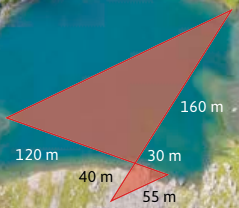
\includegraphics{Images/lagoP}
    \captionof{figure}{\small Vista fotográfica superior de la superficie del lago.}
    \label{fig:lagoP}
\end{minipage}
